\documentclass{article}[12pt]
\usepackage{fontspec}   %加這個就可以設定字體
\usepackage{xeCJK}       %讓中英文字體分開設置
\usepackage{indentfirst}
\usepackage{listings}
\usepackage[newfloat]{minted}
\usepackage{float}
\usepackage{graphicx}
\usepackage{caption}
\usepackage{fancyhdr}
\usepackage{hyperref}
\usepackage{amsmath}
\usepackage{multirow}
\usepackage[dvipsnames]{xcolor}
\usepackage{graphicx}
\usepackage{tabularx}


\usepackage[breakable, listings, skins, minted]{tcolorbox}
\usepackage{etoolbox}

\renewtcblisting{minted}{%
    listing engine=minted,
    minted language=python,
    listing only,
    breakable,
    enhanced,
    minted options = {
        linenos, 
        breaklines=true, 
        breakbefore=., 
        % fontsize=\footnotesize, 
        numbersep=2mm
    },
    overlay={%
        \begin{tcbclipinterior}
            \fill[gray!25] (frame.south west) rectangle ([xshift=4mm]frame.north west);
        \end{tcbclipinterior}
    }   
}

\usepackage[
  top=2cm,
  bottom=2cm,
  left=2cm,
  right=2cm,
  headheight=17pt, % as per the warning by fancyhdr
  includehead,includefoot,
  heightrounded, % to avoid spurious underfull messages
]{geometry} 

\newenvironment{code}{\captionsetup{type=listing}}{}
\SetupFloatingEnvironment{listing}{name=Code}


\title{Introduction to Artificial Intelligence HW 1 Report}
\author{110550088 李杰穎}
\date{\today}

\setCJKmainfont{Noto Serif CJK TC}
\setmonofont[Mapping=tex-text]{Cascadia Code}

\XeTeXlinebreaklocale "zh"             %這兩行一定要加,中文才能自動換行
\XeTeXlinebreakskip = 0pt plus 1pt     %這兩行一定要加,中文才能自動換行

\setlength{\parindent}{0em}
\setlength{\parskip}{2em}
\renewcommand{\baselinestretch}{1.5}
\begin{document}

\maketitle

\section{Code and Explanation}
\begin{code}
\captionof{listing}{Part 1 (\texttt{datasets.py})}
\begin{minted}
import os
import cv2
import numpy as np
def loadImages(dataPath):
    """
    Load all Images in the folder and transfer a list of tuples. 
    The first element is the numpy array of shape (m, n) representing the image.
    (remember to resize and convert the parking space images to 36 x 16 grayscale images.) 
    The second element is its classification (1 or 0)
        Parameters:
        dataPath: The folder path.
        Returns:
        dataset: The list of tuples.
    """
    # Begin your code (Part 1)
    dataset = [] # Declare an empty list to save the grayscale images

    # Process images in "car" directory
    for item in os.listdir(os.path.join(dataPath, "car")): # Use os.path.join to generate paths
        img = cv2.imread(os.path.join(dataPath, "car", item)) # Read image from files
        img = cv2.resize(img, (36, 16)) # Resize the image from (360, 160) to (36, 16)
        img = cv2.cvtColor(img, cv2.COLOR_BGR2GRAY) # Convert image to grayscale image
        data = (img, 1) # Create a tuple to store image and label and 
        # because all images in "car" folder is the occupied parking space, the label is set to 1
        dataset.append(data) # Append the tuple to the dataset list
    
    for item in os.listdir(os.path.join(dataPath, "non-car")): # Do the same thing as above but this time is for "non-car" folder
        img = cv2.imread(os.path.join(dataPath, "non-car", item))
        img = cv2.resize(img, (36, 16))
        img = cv2.cvtColor(img, cv2.COLOR_BGR2GRAY)
        data = (img, 0) # Not occupied parking space, label is set to 0
        dataset.append(data)
    # End your code (Part 1)
    
    return dataset

\end{minted}
\end{code}

\begin{code}
\captionof{listing}{Part 2 (\texttt{adaboost.py/selectBest})}
\begin{minted}
def selectBest(self, featureVals, iis, labels, features, weights):
"""
Finds the appropriate weak classifier for each feature.
Selects the best weak classifier for the given weights.
    Parameters:
    featureVals: A numpy array of shape (len(features), len(dataset)).
        Each row represents the values of a single feature for each training sample.
    iis: A list of numpy array with shape (m, n) representing the integral images.
    labels: A list of integer.
        The ith element is the classification of the ith training sample.
    features: A numpy array of HaarFeature class.
    weights: A numpy array with shape(len(dataset)).
        The ith element is the weight assigned to the ith training sample.
    Returns:
    bestClf: The best WeakClassifier Class
    bestError: The error of the best classifer
"""
# Begin your code (Part 2)
# Init. WeakClassifier by the feature in features list
# And append them all into the clfs list
clfs = [WeakClassifier(feature=feature) for feature in features]

# Declare bestClf and bestError to store the currently best classifier and its error
bestClf = None
bestError = sum(weights) # The max error is the sum of weights

for clf in clfs: # Iterate all classifer in clfs
    error = 0    # Declare a variable to track the error of the current clf
    for i in range(len(iis)): # Iterate all image sample
        if clf.classify(iis[i]) != labels[i]: # When the prediction of the model is different with the lable
            error += weights[i] # Add weights to error
    if error < bestError: # If the error is smaller than the best error, then classifier is the currently best classifer
        bestError = error # Change bestError to current error
        bestClf = clf     # Save this classifier as bestClf

# End your code (Part 2)
return bestClf, bestError
\end{minted}
\end{code}

\begin{code}
\captionof{listing}{Part 3 (\texttt{main.py})}
\begin{minted}
print('Start training your classifier')
for t in range(1, 11):
    print(f"Training with T={t}")
    clf = adaboost.Adaboost(T=t)
    clf.train(trainData)
    clf.save(f'clf_300_{t}')
    clf = adaboost.Adaboost.load(f'clf_300_{t}')

    print('\nEvaluate your classifier with training dataset')
    utils.evaluate(clf, trainData)

    print('\nEvaluate your classifier with test dataset')
    utils.evaluate(clf, testData)

    # Part 4: Implement detect function in detection.py and test the following code.
    print('\nUse your classifier with video.gif to get the predictions (one .txt and one .png)')
    detection.detect('data/detect/detectData.txt', clf, t)
\end{minted}
\end{code}

\begin{code}
\captionof{listing}{Part 4 (\texttt{detection.py/detect})}
\begin{minted}
def detect(dataPath, clf, t=10):
    """
    Please read detectData.txt to understand the format. 
    Use cv2.VideoCapture() to load the video.gif.
    Use crop() to crop each frame (frame size = 1280 x 800) of video to get parking space images. (image size = 360 x 160) 
    Convert each parking space image into 36 x 16 and grayscale.
    Use clf.classify() function to detect car, If the result is True, draw the green box on the image like the example provided on the spec. 
    Then, you have to show the first frame with the bounding boxes in your report.
    Save the predictions as .txt file (Adaboost_pred.txt), the format is the same as GroundTruth.txt. 
    (in order to draw the plot in Yolov5_sample_code.ipynb)
    
      Parameters:
        dataPath: the path of detectData.txt
      Returns:
        No returns.
    """
    # Begin your code (Part 4)
    cords = []
    with open(dataPath) as file:
        num_of_parking = int(file.readline())
        for _ in range(num_of_parking):
            tmp = file.readline()
            tmp = tmp.split(" ")
            res = tuple(map(int, tmp))
            cords.append(res)
    cap = cv2.VideoCapture(os.path.join(dataPath, "..", "video.gif"))
    frame = 0
    output_gif = []
    first_frame = True
    while True:
        detect_label = []
        frame += 1
        print(f"frame: {frame}")
        _, img = cap.read()
        if img is None:
            break
        for cord in cords:
            pic = crop(*cord, img)
            pic = cv2.resize(pic, (36, 16))
            pic = cv2.cvtColor(pic, cv2.COLOR_RGB2GRAY)
            detect_label.append(clf.classify(pic))
        for i, label in enumerate(detect_label):
            if label:
                pos = [[cords[i][idx], cords[i][idx+1]] for idx in range(0, 8, 2)]
                pos[2], pos[3] = pos[3], pos[2]
                pos = np.array(pos, np.int32)
                cv2.polylines(img, [pos], color=(0, 255, 0), isClosed=True)
    
        output_gif.append(cv2.cvtColor(img, cv2.COLOR_BGR2RGB))
        if first_frame:
            first_frame = False
            cv2.imwrite(f"Adaboost_first_frame_{t}.png", img)
        with open(f"Adaboost_pred_{t}.txt", "a") as txt:
            res = ""
            for i, label in enumerate(detect_label):
                if label:
                    res += "1"
                else:
                    res += "0"
                if i != len(detect_label) - 1:
                    res += " "
                else:
                    res += "\n"
            txt.write(res)
    imageio.mimsave(f'results_{t}.gif', output_gif, fps=2)
\end{minted}
\end{code}

\begin{code}
\captionof{listing}{Part 5 (\texttt{yolov5\_sample\_code.ipynb})}
\begin{minted}
dataPath = os.path.join("HW1_material", "detect", "detectData.txt")
cords = []
with open(dataPath) as file:
    num_of_parking = int(file.readline())
    for _ in range(num_of_parking):
        tmp = file.readline()
        tmp = tmp.split(" ")
        res = tuple(map(int, tmp))
        cords.append(res)
cap = cv2.VideoCapture(os.path.join("HW1_material", "detect", "video.gif"))
frame = 0
output_gif = []
first_frame = True
while True:
    detect_label = []
    frame += 1
    print(f"frame: {frame}")
    _, img = cap.read()
    if img is None:
        break
    for cord in cords:
        pic = crop(*cord, img)
        pic = cv2.resize(pic, (36, 16))
        detect_label.append(yolov5_func.classify(pic, weight_path, confidence_threshold, (36, 16)))
    for i, label in enumerate(detect_label):
        if label:
            pos = [[cords[i][idx], cords[i][idx+1]] for idx in range(0, 8, 2)]
            pos[2], pos[3] = pos[3], pos[2]
            pos = np.array(pos, np.int32)
            cv2.polylines(img, [pos], color=(0, 255, 0), isClosed=True)
    if first_frame:
        cv2.imwrite(img_save_path, img)
        first_frame = False
    output_gif.append(cv2.cvtColor(img, cv2.COLOR_BGR2RGB))
    with open(txt_save_path, "a") as txt:
        res = ""
        for i, label in enumerate(detect_label):
            if label:
                res += "1"
            else:
                res += "0"
            if i != len(detect_label) - 1:
                res += " "
            else:
                res += "\n"
        txt.write(res)
imageio.mimsave(f'results.gif', output_gif, fps=2)
\end{minted}
\end{code}

\section{Experiments}
\subsection{Hyperparameters Adjustment}
\subsubsection{Adaboost}
In Adaboost algorithm, the only hyperparameter we can change is \texttt{T}, 
which indicates the number of classifers that will be used in the training process.

\subsection{YOLOv5}


\subsubsection{YOLOv5}
\section{Results}
\subsection{Measurements}
\subsubsection{Accuracy}
In binary classification problem, we often define four kinds of accuracy, 
which are True Positive, True Negative, False Positive and False Negative 
to show the performance of classifiers. Their definitions are written below:
\begin{itemize}
    \item True Positive (TP): The real label is \textbf{true}, 
    and our model predicts that it's \textbf{true}.
    \item True Negative (TN): The real label is \textbf{false}, 
    and our model predicts that it's \textbf{false}.
    \item False Positive (FP): The real label is \textbf{true}, 
    but our model predicts that it's \textbf{false}.
    \item False Negative (FN): The real label is \textbf{false}, 
    but our model predicts that it's \textbf{true}.
\end{itemize}
\subsubsection{F-Score}
F-score is used to measure a test's accuracy. 
To define F-score, we first need to define two variables, 
``precision'' and ``recall''.

\begin{equation}
    \text {precision}=\frac{\text{TP}}{\text{TP}+\text{FP}}
\end{equation}

\begin{equation}
    \text {recall}=\frac{\text{TP}}{\text{TP}+\text{FN}}
\end{equation}

And the definition of F-score is:

\begin{equation}
    \text {F-score}=\frac{\left(1+\beta^{2}\right) \text { precision } \times \text { recall }}{\beta^{2} \text { precision }+\text { recall }}
\end{equation}

In reality, we often use ``F1-score'', which means $\beta=1$. So the ``F1-score'' can be written as:
\begin{equation}
    \text {F1-score}=2 \times \frac{\text { precision } \times \text { recall }}{\text { precision }+\text { recall }}
\end{equation}

The range of F1-score is $[0, 1]$. If F1-score is higher (closer to 1), 
then the performance of classifer is better.




\subsection{Visuals Results}



\begin{figure}[H]
    \centering
    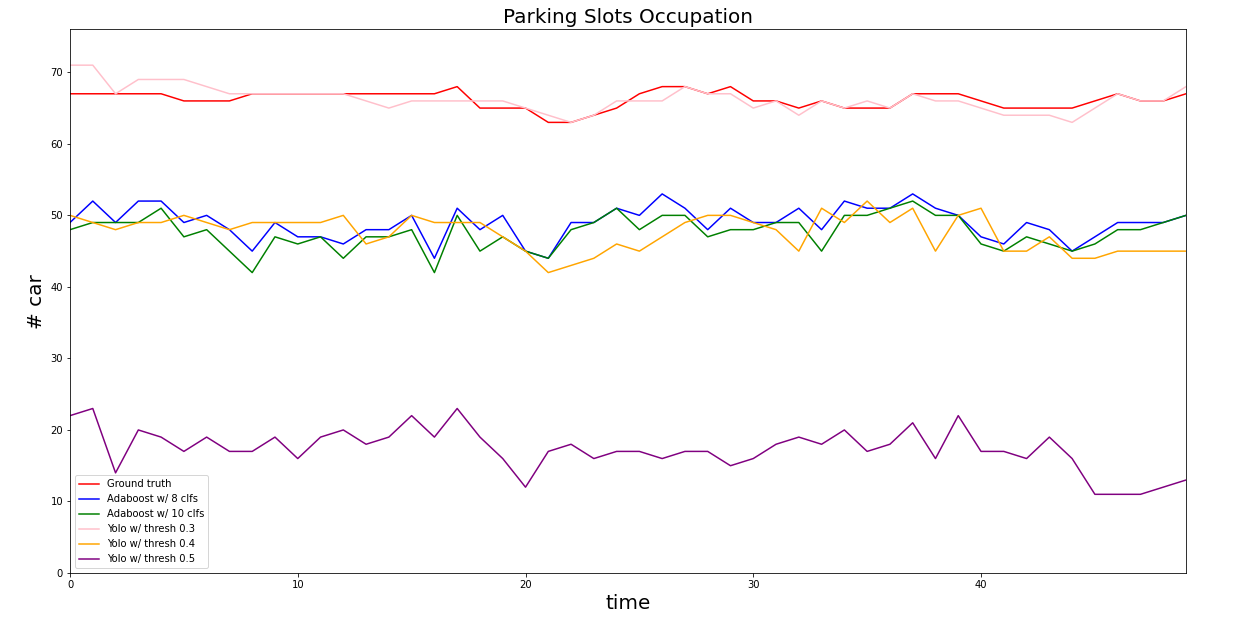
\includegraphics[width=\textwidth]{figure/Parking_Slots_Occupation.png}
    \caption{The number of occupied parking slots detected by Adaboost(with 8 and 10 classifers)
    , YOLOv5(with threshold 0.3, 0.4 and 0.5) and the ground truth}
\end{figure}

We use equation \ref{eq:acc} to calculate the accuracy in figure \ref{fig:acc}.
\begin{equation}
    \text{Accuracy} = \frac{\text{TP}+\text{TN}}{\text{Total}}
    \label{eq:acc}
\end{equation}

\begin{figure}[H]
    \centering
    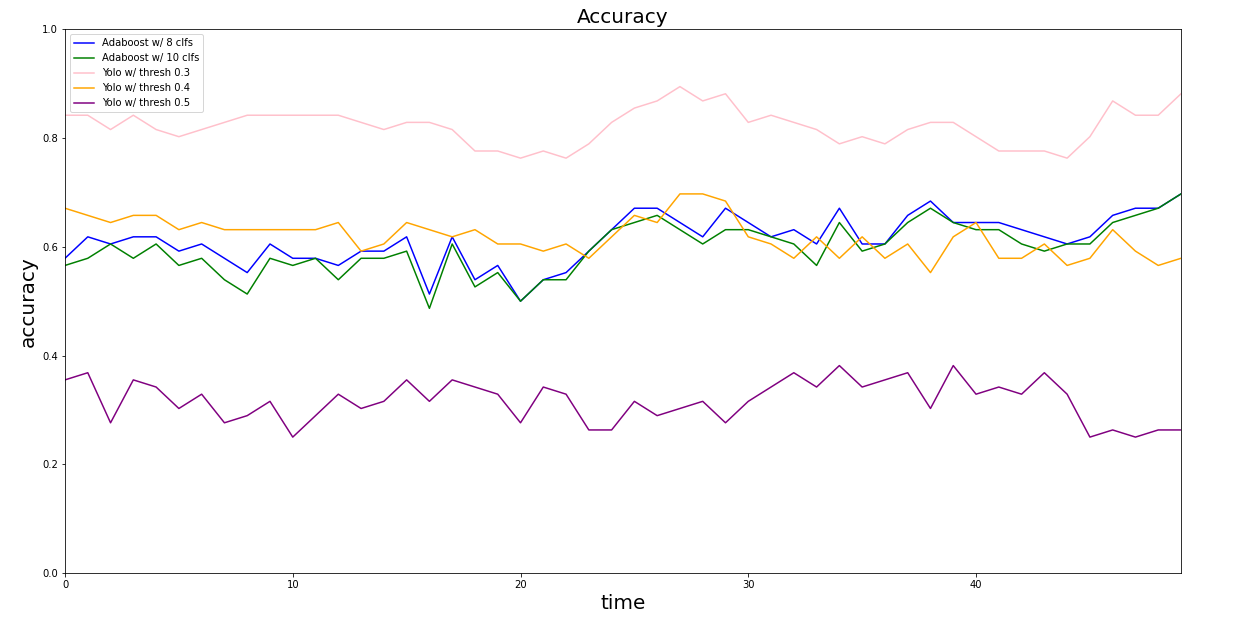
\includegraphics[width=\textwidth]{figure/Accuracy.png}
    \caption{Accuracy of Adaboost (w/ 8 and 10 classifers)
    and YOLOv5 (w/ threshold 0.3, 0.4 and 0.5) over time}
    \label{fig:acc}
\end{figure}


\begin{figure}[H]
    \centering
    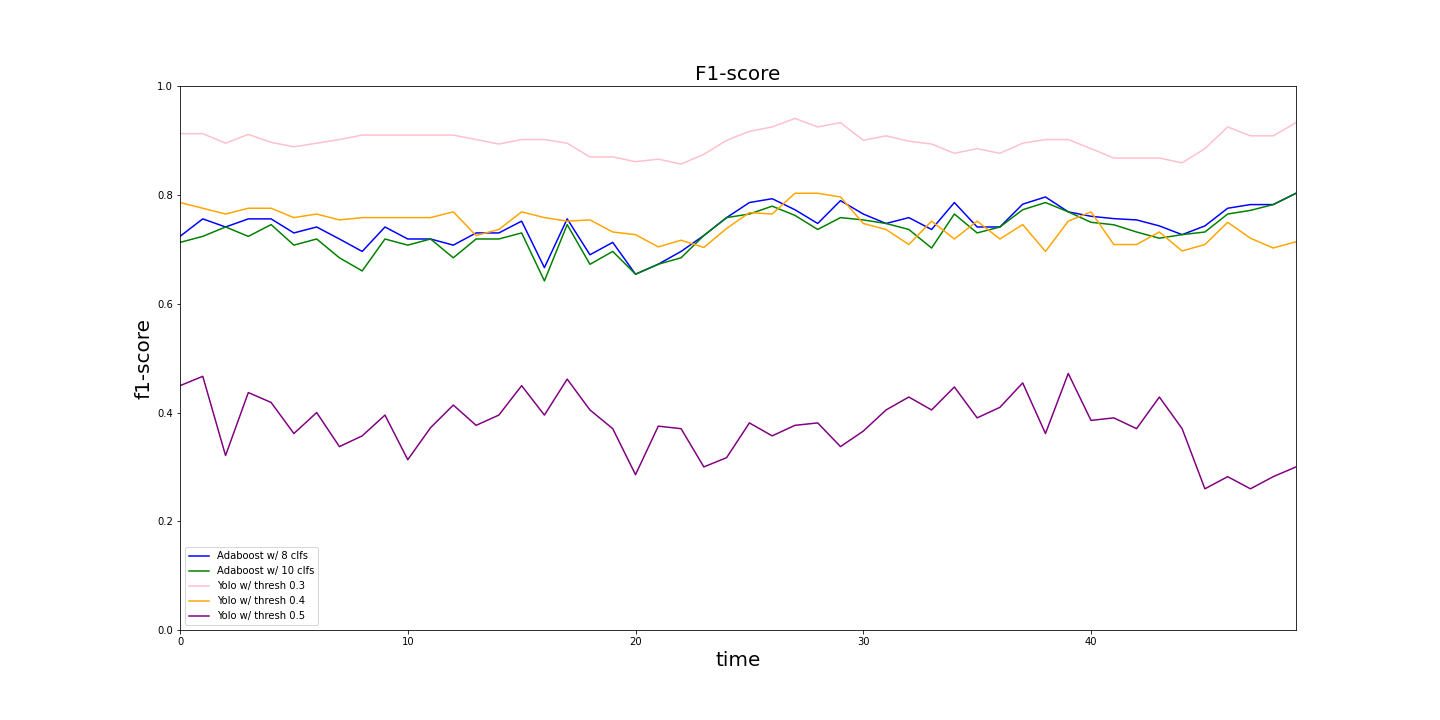
\includegraphics[width=\textwidth]{figure/F1-score.png}
    \caption{F1-score of Adaboost (w/ 8 and 10 classifers)
    and YOLOv5 (w/ threshold 0.3, 0.4 and 0.5) over time}
    \label{fig:F1}
\end{figure}

\begin{figure}[H]
    \centering
    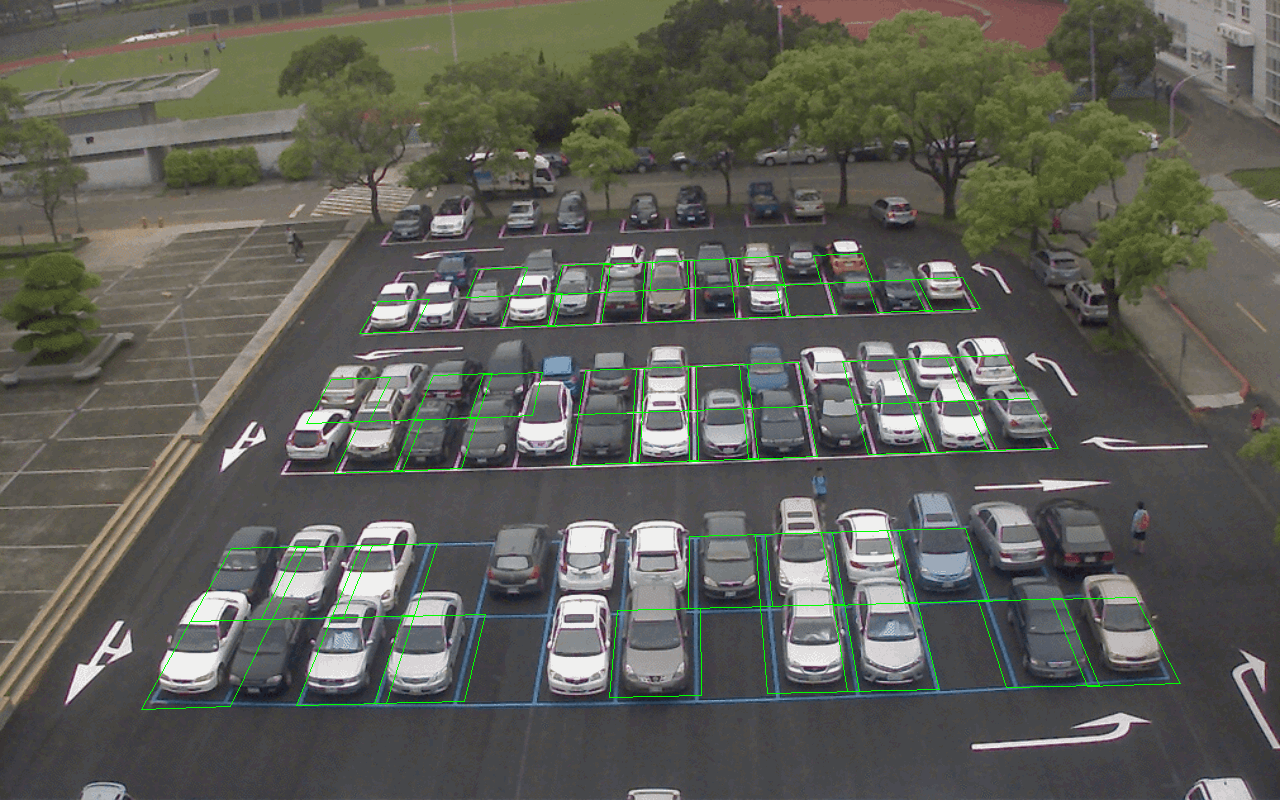
\includegraphics[width=0.75\textwidth]{figure/Adaboost_first_frame_8.png}
    \caption{The detection result of Adaboost with 8 classfiers}
\end{figure}

\begin{figure}[H]
    \centering
    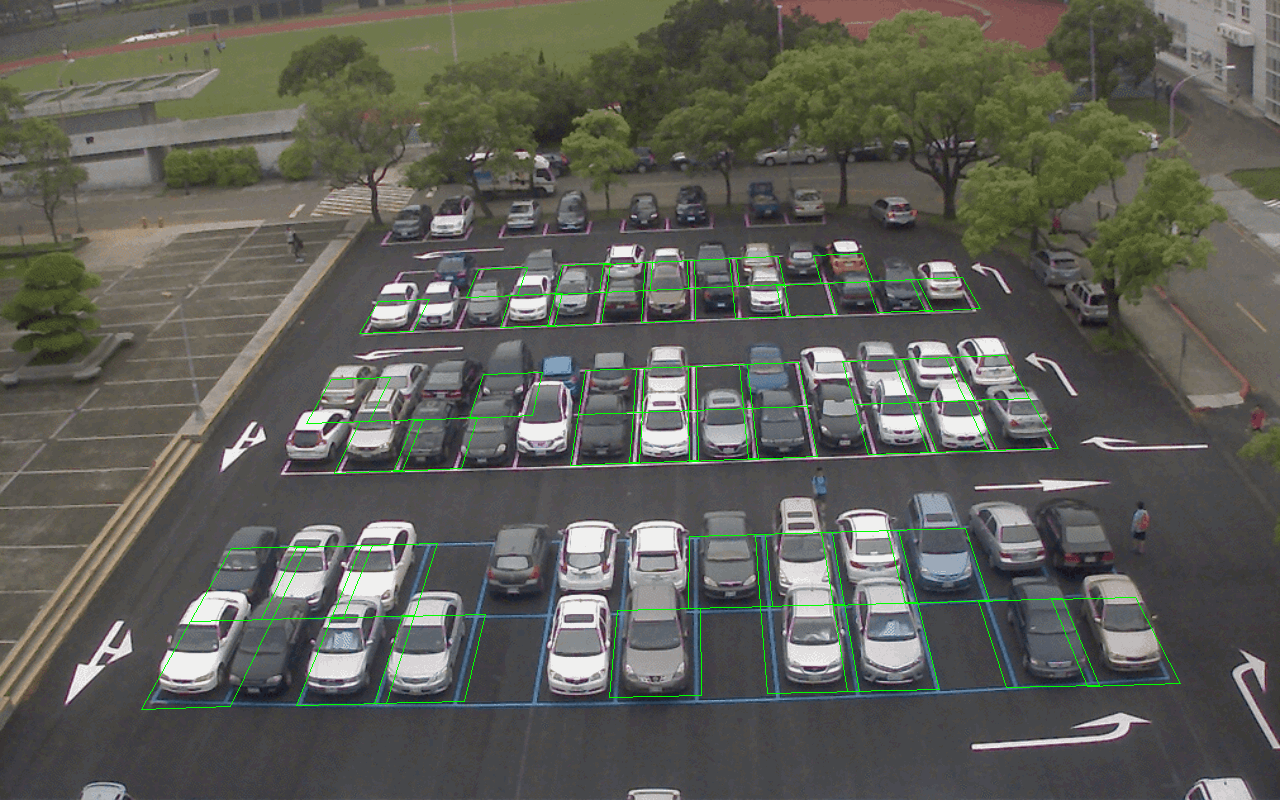
\includegraphics[width=0.75\textwidth]{figure/Adaboost_first_frame_10.png}
    \caption{The detection result of Adaboost with 10 classfiers}
\end{figure}

\begin{figure}[H]
    \centering
    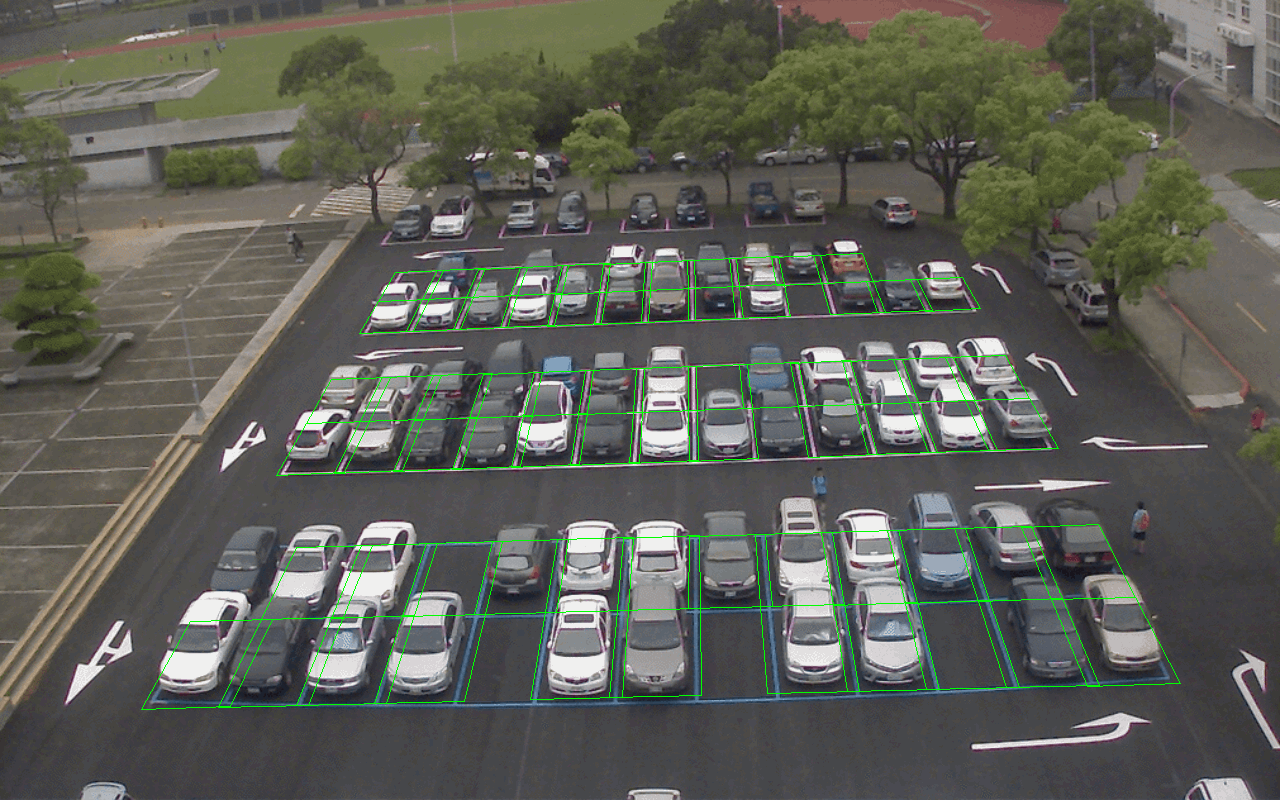
\includegraphics[width=0.75\textwidth]{figure/Yolov5_first_frame_3.png}
    \caption{The detection result of YOLOv5 with threshold set to 0.3}
\end{figure}


\begin{figure}[H]
    \centering
    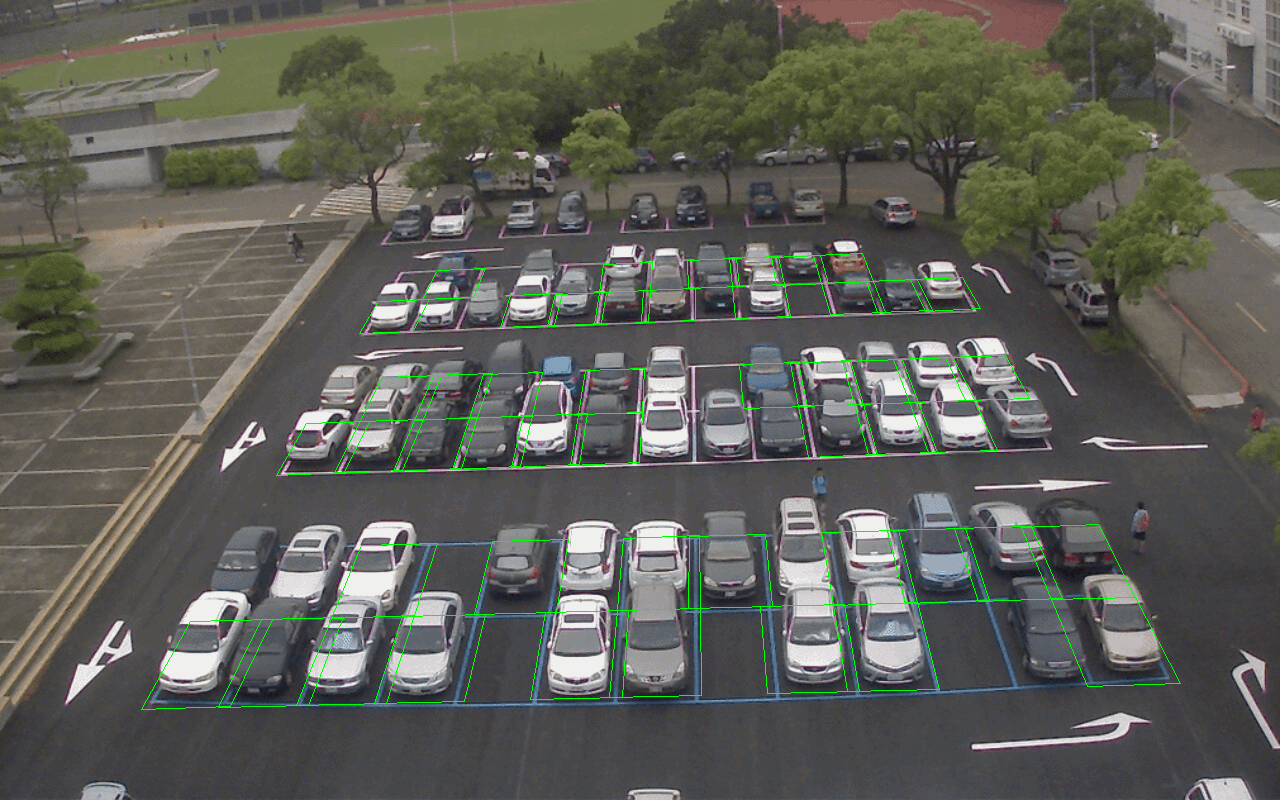
\includegraphics[width=0.75\textwidth]{figure/Yolov5_first_frame_4.png}
    \caption{The detection result of YOLOv5 with threshold set to 0.4}
\end{figure}


\begin{figure}[H]
    \centering
    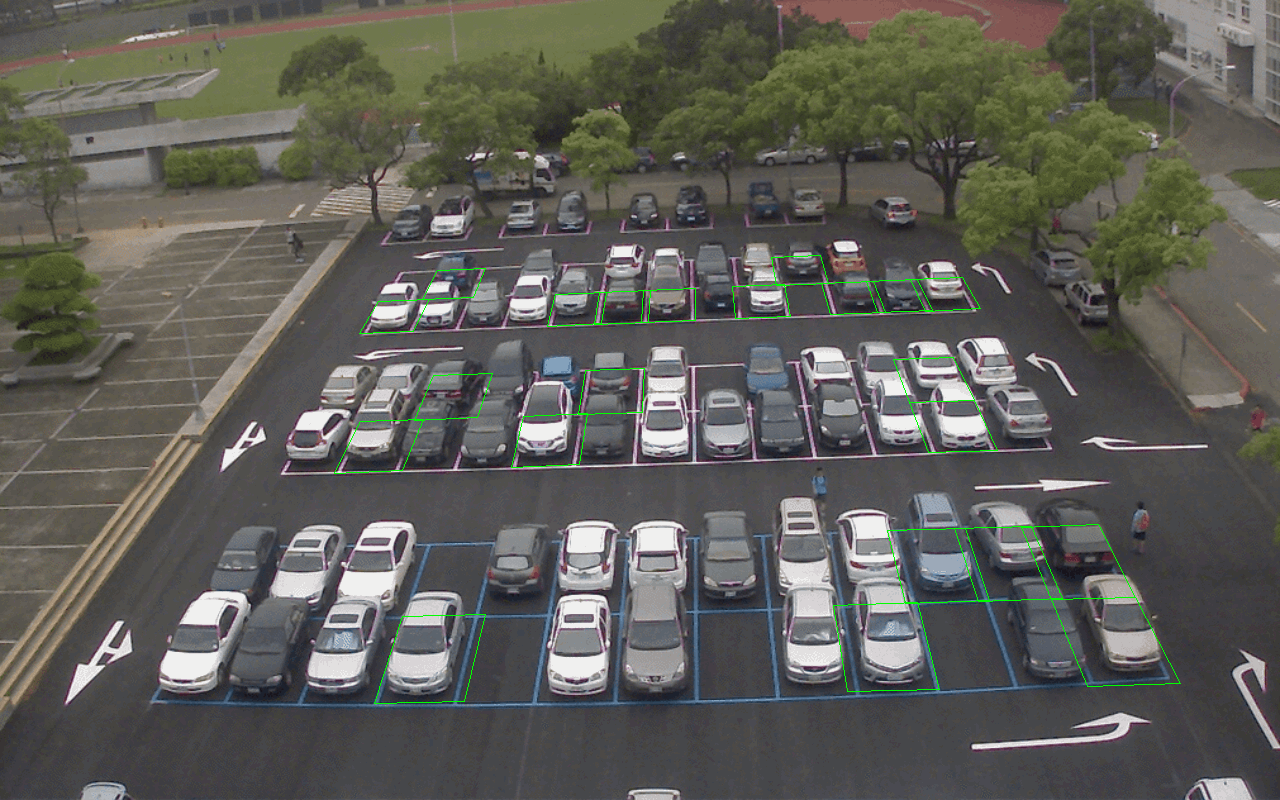
\includegraphics[width=0.75\textwidth]{figure/Yolov5_first_frame_5.png}
    \caption{The detection result of YOLOv5 with threshold set to 0.5}
\end{figure}



\section{Problems}
\subsection{alpha = math.log(1.0/beta) ValueError: math domain error}
\subsection{The model has bad performance}



\end{document}